% Created by tikzDevice version 0.9 on 2015-12-16 01:29:24
% !TEX encoding = UTF-8 Unicode
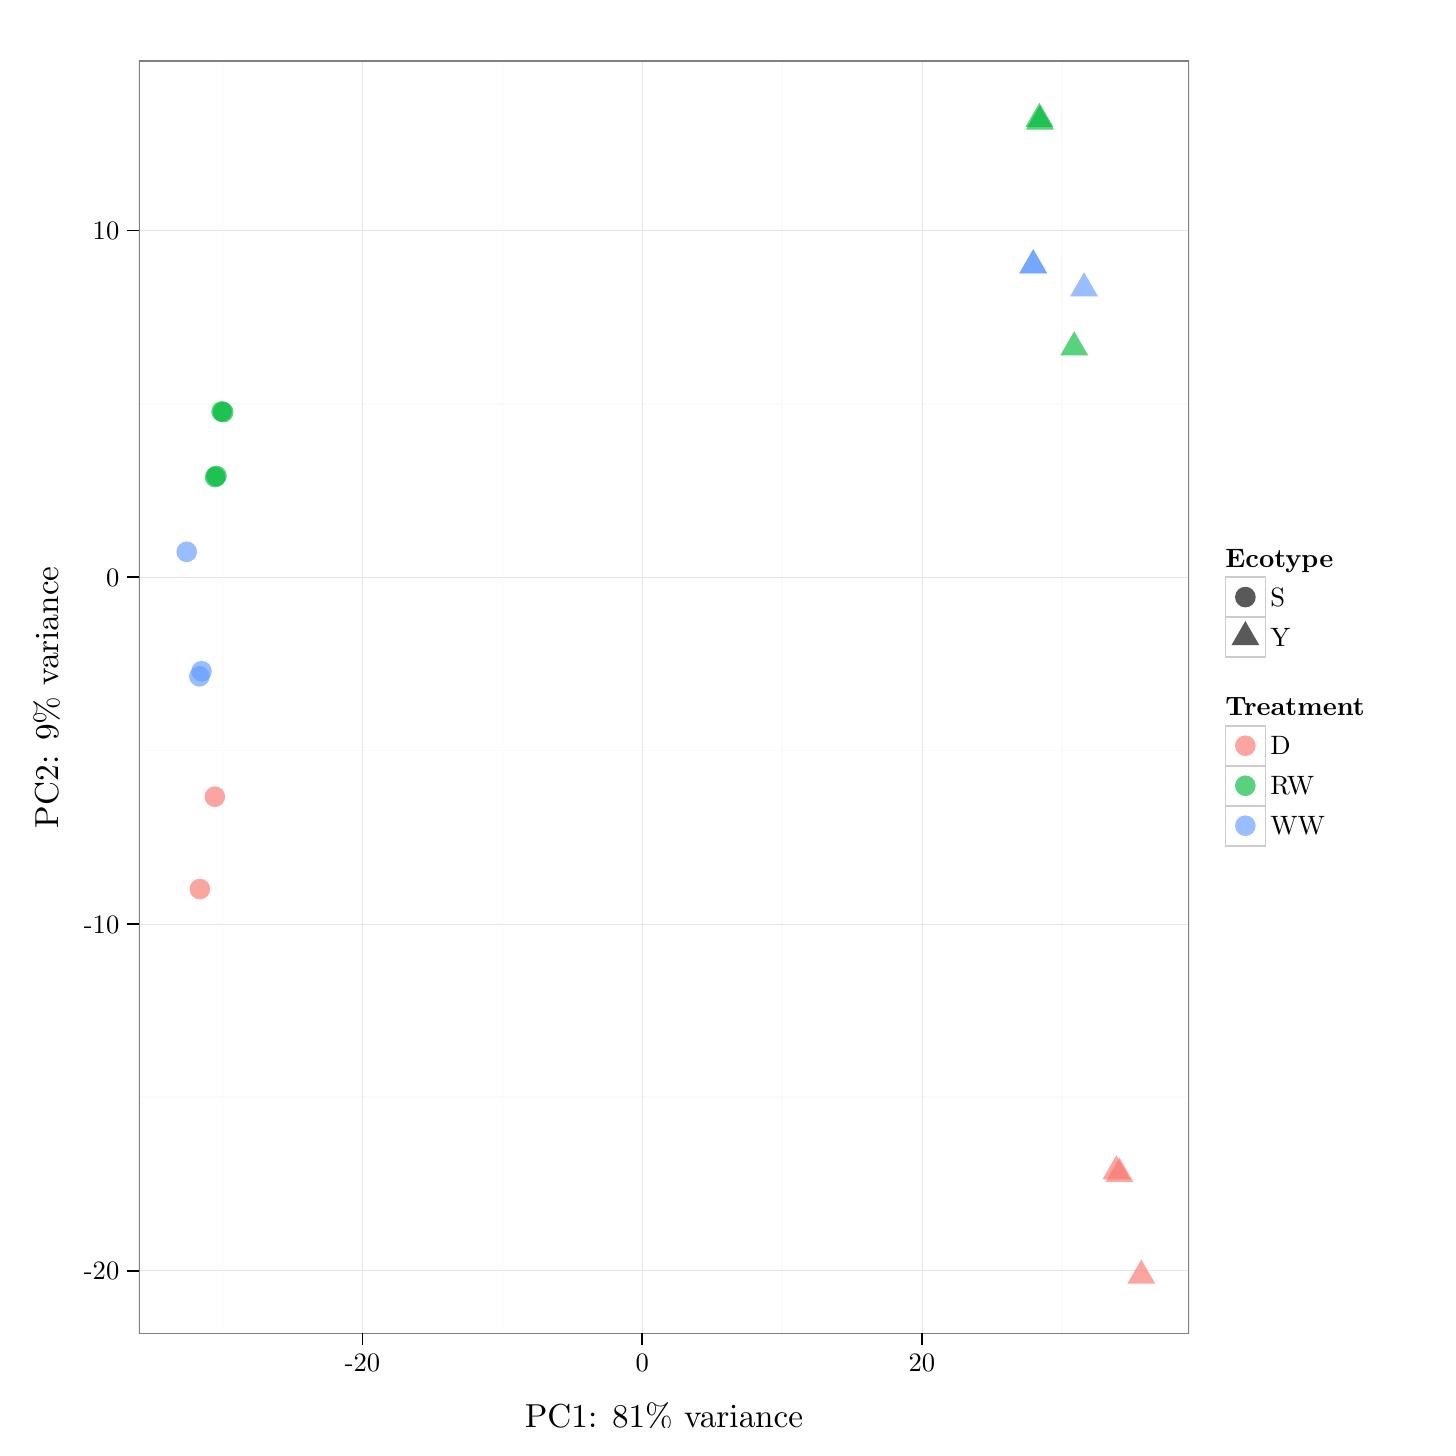
\begin{tikzpicture}[x=1pt,y=1pt]
\definecolor{fillColor}{RGB}{255,255,255}
\path[use as bounding box,fill=fillColor,fill opacity=0.00] (0,0) rectangle (505.89,505.89);
\begin{scope}
\path[clip] (  0.00,  0.00) rectangle (505.89,505.89);
\definecolor{drawColor}{RGB}{255,255,255}
\definecolor{fillColor}{RGB}{255,255,255}

\path[draw=drawColor,line width= 0.6pt,line join=round,line cap=round,fill=fillColor] (  0.00,  0.00) rectangle (505.89,505.89);
\end{scope}
\begin{scope}
\path[clip] ( 40.22, 34.03) rectangle (419.65,493.85);
\definecolor{fillColor}{RGB}{255,255,255}

\path[fill=fillColor] ( 40.22, 34.03) rectangle (419.65,493.85);
\definecolor{drawColor}{gray}{0.98}

\path[draw=drawColor,line width= 0.6pt,line join=round] ( 40.22,119.38) --
	(419.65,119.38);

\path[draw=drawColor,line width= 0.6pt,line join=round] ( 40.22,244.68) --
	(419.65,244.68);

\path[draw=drawColor,line width= 0.6pt,line join=round] ( 40.22,369.97) --
	(419.65,369.97);

\path[draw=drawColor,line width= 0.6pt,line join=round] ( 70.46, 34.03) --
	( 70.46,493.85);

\path[draw=drawColor,line width= 0.6pt,line join=round] (171.53, 34.03) --
	(171.53,493.85);

\path[draw=drawColor,line width= 0.6pt,line join=round] (272.60, 34.03) --
	(272.60,493.85);

\path[draw=drawColor,line width= 0.6pt,line join=round] (373.67, 34.03) --
	(373.67,493.85);
\definecolor{drawColor}{gray}{0.90}

\path[draw=drawColor,line width= 0.2pt,line join=round] ( 40.22, 56.73) --
	(419.65, 56.73);

\path[draw=drawColor,line width= 0.2pt,line join=round] ( 40.22,182.03) --
	(419.65,182.03);

\path[draw=drawColor,line width= 0.2pt,line join=round] ( 40.22,307.32) --
	(419.65,307.32);

\path[draw=drawColor,line width= 0.2pt,line join=round] ( 40.22,432.62) --
	(419.65,432.62);

\path[draw=drawColor,line width= 0.2pt,line join=round] (121.00, 34.03) --
	(121.00,493.85);

\path[draw=drawColor,line width= 0.2pt,line join=round] (222.06, 34.03) --
	(222.06,493.85);

\path[draw=drawColor,line width= 0.2pt,line join=round] (323.13, 34.03) --
	(323.13,493.85);
\definecolor{fillColor}{RGB}{248,118,109}

\path[fill=fillColor,fill opacity=0.65] ( 62.23,194.62) circle (  3.73);

\path[fill=fillColor,fill opacity=0.65] ( 67.64,227.99) circle (  3.73);
\definecolor{fillColor}{RGB}{0,186,56}

\path[fill=fillColor,fill opacity=0.65] ( 70.65,366.95) circle (  3.73);

\path[fill=fillColor,fill opacity=0.65] ( 70.09,367.21) circle (  3.73);

\path[fill=fillColor,fill opacity=0.65] ( 67.73,343.47) circle (  3.73);

\path[fill=fillColor,fill opacity=0.65] ( 68.22,343.90) circle (  3.73);
\definecolor{fillColor}{RGB}{97,156,255}

\path[fill=fillColor,fill opacity=0.65] ( 57.47,316.49) circle (  3.73);

\path[fill=fillColor,fill opacity=0.65] ( 62.82,273.33) circle (  3.73);

\path[fill=fillColor,fill opacity=0.65] ( 62.05,271.50) circle (  3.73);
\definecolor{fillColor}{RGB}{248,118,109}

\path[fill=fillColor,fill opacity=0.65] (402.40, 60.74) --
	(407.43, 52.03) --
	(397.37, 52.03) --
	cycle;

\path[fill=fillColor,fill opacity=0.65] (393.39, 98.43) --
	(398.42, 89.72) --
	(388.36, 89.72) --
	cycle;

\path[fill=fillColor,fill opacity=0.65] (394.52, 97.54) --
	(399.55, 88.83) --
	(389.49, 88.83) --
	cycle;
\definecolor{fillColor}{RGB}{0,186,56}

\path[fill=fillColor,fill opacity=0.65] (378.17,396.18) --
	(383.20,387.47) --
	(373.14,387.47) --
	cycle;

\path[fill=fillColor,fill opacity=0.65] (365.78,477.78) --
	(370.81,469.07) --
	(360.75,469.07) --
	cycle;

\path[fill=fillColor,fill opacity=0.65] (365.59,478.75) --
	(370.62,470.04) --
	(360.56,470.04) --
	cycle;
\definecolor{fillColor}{RGB}{97,156,255}

\path[fill=fillColor,fill opacity=0.65] (381.72,417.51) --
	(386.75,408.80) --
	(376.69,408.80) --
	cycle;

\path[fill=fillColor,fill opacity=0.65] (363.33,425.85) --
	(368.36,417.14) --
	(358.30,417.14) --
	cycle;

\path[fill=fillColor,fill opacity=0.65] (363.36,425.85) --
	(368.39,417.14) --
	(358.33,417.14) --
	cycle;
\definecolor{drawColor}{gray}{0.50}

\path[draw=drawColor,line width= 0.6pt,line join=round,line cap=round] ( 40.22, 34.03) rectangle (419.65,493.85);
\end{scope}
\begin{scope}
\path[clip] (  0.00,  0.00) rectangle (505.89,505.89);
\definecolor{drawColor}{RGB}{0,0,0}

\node[text=drawColor,anchor=base east,inner sep=0pt, outer sep=0pt, scale=  0.96] at ( 33.11, 53.42) {-20};

\node[text=drawColor,anchor=base east,inner sep=0pt, outer sep=0pt, scale=  0.96] at ( 33.11,178.72) {-10};

\node[text=drawColor,anchor=base east,inner sep=0pt, outer sep=0pt, scale=  0.96] at ( 33.11,304.02) {0};

\node[text=drawColor,anchor=base east,inner sep=0pt, outer sep=0pt, scale=  0.96] at ( 33.11,429.32) {10};
\end{scope}
\begin{scope}
\path[clip] (  0.00,  0.00) rectangle (505.89,505.89);
\definecolor{drawColor}{RGB}{0,0,0}

\path[draw=drawColor,line width= 0.6pt,line join=round] ( 35.95, 56.73) --
	( 40.22, 56.73);

\path[draw=drawColor,line width= 0.6pt,line join=round] ( 35.95,182.03) --
	( 40.22,182.03);

\path[draw=drawColor,line width= 0.6pt,line join=round] ( 35.95,307.32) --
	( 40.22,307.32);

\path[draw=drawColor,line width= 0.6pt,line join=round] ( 35.95,432.62) --
	( 40.22,432.62);
\end{scope}
\begin{scope}
\path[clip] (  0.00,  0.00) rectangle (505.89,505.89);
\definecolor{drawColor}{RGB}{0,0,0}

\path[draw=drawColor,line width= 0.6pt,line join=round] (121.00, 29.77) --
	(121.00, 34.03);

\path[draw=drawColor,line width= 0.6pt,line join=round] (222.06, 29.77) --
	(222.06, 34.03);

\path[draw=drawColor,line width= 0.6pt,line join=round] (323.13, 29.77) --
	(323.13, 34.03);
\end{scope}
\begin{scope}
\path[clip] (  0.00,  0.00) rectangle (505.89,505.89);
\definecolor{drawColor}{RGB}{0,0,0}

\node[text=drawColor,anchor=base,inner sep=0pt, outer sep=0pt, scale=  0.96] at (121.00, 20.31) {-20};

\node[text=drawColor,anchor=base,inner sep=0pt, outer sep=0pt, scale=  0.96] at (222.06, 20.31) {0};

\node[text=drawColor,anchor=base,inner sep=0pt, outer sep=0pt, scale=  0.96] at (323.13, 20.31) {20};
\end{scope}
\begin{scope}
\path[clip] (  0.00,  0.00) rectangle (505.89,505.89);
\definecolor{drawColor}{RGB}{0,0,0}

\node[text=drawColor,anchor=base,inner sep=0pt, outer sep=0pt, scale=  1.20] at (229.93,  0) {PC1: 81\% variance};
\end{scope}
\begin{scope}
\path[clip] (  0.00,  0.00) rectangle (505.89,505.89);
\definecolor{drawColor}{RGB}{0,0,0}

\node[text=drawColor,rotate= 90.00,anchor=base,inner sep=0pt, outer sep=0pt, scale=  1.20] at ( 11,263.94) {PC2: 9\% variance};
\end{scope}
\begin{scope}
\path[clip] (  0.00,  0.00) rectangle (505.89,505.89);
\definecolor{fillColor}{RGB}{255,255,255}

\path[fill=fillColor] (428.51,274.18) rectangle (473.84,321.86);
\end{scope}
\begin{scope}
\path[clip] (  0.00,  0.00) rectangle (505.89,505.89);
\definecolor{drawColor}{RGB}{0,0,0}

\node[text=drawColor,anchor=base west,inner sep=0pt, outer sep=0pt, scale=  0.96] at (432.78,310.97) {\bfseries Ecotype};
\end{scope}
\begin{scope}
\path[clip] (  0.00,  0.00) rectangle (505.89,505.89);
\definecolor{drawColor}{gray}{0.80}
\definecolor{fillColor}{RGB}{255,255,255}

\path[draw=drawColor,line width= 0.6pt,line join=round,line cap=round,fill=fillColor] (432.78,292.90) rectangle (447.23,307.35);
\end{scope}
\begin{scope}
\path[clip] (  0.00,  0.00) rectangle (505.89,505.89);
\definecolor{fillColor}{RGB}{0,0,0}

\path[fill=fillColor,fill opacity=0.65] (440.01,300.13) circle (  3.73);
\end{scope}
\begin{scope}
\path[clip] (  0.00,  0.00) rectangle (505.89,505.89);
\definecolor{drawColor}{gray}{0.80}
\definecolor{fillColor}{RGB}{255,255,255}

\path[draw=drawColor,line width= 0.6pt,line join=round,line cap=round,fill=fillColor] (432.78,278.45) rectangle (447.23,292.90);
\end{scope}
\begin{scope}
\path[clip] (  0.00,  0.00) rectangle (505.89,505.89);
\definecolor{fillColor}{RGB}{0,0,0}

\path[fill=fillColor,fill opacity=0.65] (440.01,291.48) --
	(445.04,282.77) --
	(434.98,282.77) --
	cycle;
\end{scope}
\begin{scope}
\path[clip] (  0.00,  0.00) rectangle (505.89,505.89);
\definecolor{drawColor}{RGB}{0,0,0}

\node[text=drawColor,anchor=base west,inner sep=0pt, outer sep=0pt, scale=  0.96] at (449.04,296.82) {S};
\end{scope}
\begin{scope}
\path[clip] (  0.00,  0.00) rectangle (505.89,505.89);
\definecolor{drawColor}{RGB}{0,0,0}

\node[text=drawColor,anchor=base west,inner sep=0pt, outer sep=0pt, scale=  0.96] at (449.04,282.37) {Y};
\end{scope}
\begin{scope}
\path[clip] (  0.00,  0.00) rectangle (505.89,505.89);
\definecolor{fillColor}{RGB}{255,255,255}

\path[fill=fillColor] (428.51,206.02) rectangle (484.98,268.16);
\end{scope}
\begin{scope}
\path[clip] (  0.00,  0.00) rectangle (505.89,505.89);
\definecolor{drawColor}{RGB}{0,0,0}

\node[text=drawColor,anchor=base west,inner sep=0pt, outer sep=0pt, scale=  0.96] at (432.78,257.26) {\bfseries Treatment};
\end{scope}
\begin{scope}
\path[clip] (  0.00,  0.00) rectangle (505.89,505.89);
\definecolor{drawColor}{gray}{0.80}
\definecolor{fillColor}{RGB}{255,255,255}

\path[draw=drawColor,line width= 0.6pt,line join=round,line cap=round,fill=fillColor] (432.78,239.20) rectangle (447.23,253.65);
\end{scope}
\begin{scope}
\path[clip] (  0.00,  0.00) rectangle (505.89,505.89);
\definecolor{fillColor}{RGB}{248,118,109}

\path[fill=fillColor,fill opacity=0.65] (440.01,246.42) circle (  3.73);
\end{scope}
\begin{scope}
\path[clip] (  0.00,  0.00) rectangle (505.89,505.89);
\definecolor{drawColor}{gray}{0.80}
\definecolor{fillColor}{RGB}{255,255,255}

\path[draw=drawColor,line width= 0.6pt,line join=round,line cap=round,fill=fillColor] (432.78,224.74) rectangle (447.23,239.20);
\end{scope}
\begin{scope}
\path[clip] (  0.00,  0.00) rectangle (505.89,505.89);
\definecolor{fillColor}{RGB}{0,186,56}

\path[fill=fillColor,fill opacity=0.65] (440.01,231.97) circle (  3.73);
\end{scope}
\begin{scope}
\path[clip] (  0.00,  0.00) rectangle (505.89,505.89);
\definecolor{drawColor}{gray}{0.80}
\definecolor{fillColor}{RGB}{255,255,255}

\path[draw=drawColor,line width= 0.6pt,line join=round,line cap=round,fill=fillColor] (432.78,210.29) rectangle (447.23,224.74);
\end{scope}
\begin{scope}
\path[clip] (  0.00,  0.00) rectangle (505.89,505.89);
\definecolor{fillColor}{RGB}{97,156,255}

\path[fill=fillColor,fill opacity=0.65] (440.01,217.51) circle (  3.73);
\end{scope}
\begin{scope}
\path[clip] (  0.00,  0.00) rectangle (505.89,505.89);
\definecolor{drawColor}{RGB}{0,0,0}

\node[text=drawColor,anchor=base west,inner sep=0pt, outer sep=0pt, scale=  0.96] at (449.04,243.12) {D};
\end{scope}
\begin{scope}
\path[clip] (  0.00,  0.00) rectangle (505.89,505.89);
\definecolor{drawColor}{RGB}{0,0,0}

\node[text=drawColor,anchor=base west,inner sep=0pt, outer sep=0pt, scale=  0.96] at (449.04,228.66) {RW};
\end{scope}
\begin{scope}
\path[clip] (  0.00,  0.00) rectangle (505.89,505.89);
\definecolor{drawColor}{RGB}{0,0,0}

\node[text=drawColor,anchor=base west,inner sep=0pt, outer sep=0pt, scale=  0.96] at (449.04,214.21) {WW};
\end{scope}
\end{tikzpicture}
